\section{The proposed platform}
\label{sec:platform}

This section describes a platform that does not exist. It is the target the proof of concept
(PoC) is one walking skeleton toward, drawn from the design already latent in the PoC's code and
decisions (\repo{docs/architecture/decisions}). Almost everything in this section is
\textsc{future work} \evfut. Every component below states its own status; a status tag of
\textsc{implemented in poc} names the file that exists today, and nothing else in this section
should be read as built. The PoC has no human validation. The gap map in
\cref{sec:n3} produces gap candidates, not identified tacit knowledge, and nothing in this
platform design changes that: a gap candidate remains a prediction until a human answers it.

\subsection{Three evidence worlds}
\label{sec:platform-worlds}

The platform organizes every piece of evidence into one of three worlds, already a typed field
in the PoC's code: \code{World.A = "public"}, \code{World.B = "organisational"},
\code{World.C = "human"} (\repo{residual/src/residual/vocab.py}) \evobs. A world is defined by
which body of evidence a source belongs to, not by how it was accessed. A public learner-response
dataset is World A even though a school collected it, and an open-source project's own commit
history is World B even though the repository is public.

\paragraph{World A --- public evidence.}
Textbooks, papers, standards, guidance, forums, task analyses, and public learner-response
datasets. It can yield concepts, taxonomies, taught heuristics, and cohort-level difficulty
\evint, but not episode-specific cues or organization-specific practice, since those are not
written down for the public. \evobs{} Implemented for open-web text only, in the two live N3
domains; no curated tier yet (every source is host tier \code{"open"}, decision 0007). Public
learner datasets are not ingested (N4, \textsc{next research stage}).

\paragraph{World B --- organization-specific evidence.}
Standard operating procedures (SOPs), wikis, tickets, commits, review threads, logs, incident reports, and design records
(\repo{residual/src/residual/vocab.py}) \evobs. World B carries a second axis World A does not
need, \emph{practice}: \code{imagined} (an SOP prescribes), \code{done} (a log records), or
\code{reported}; the gap between imagined and done is the organizational form of the residual
\evhyp. The schema exists \evobs; no ingestion does. The only planned adapter is a Git-history
adapter over \emph{public} repositories for the H-OSS study (V3, \cref{subsec:hoss}), \textsc{next research stage}; customer or
employee data is \textsc{long-term}, gated on a DPIA (\cref{sec:platform-nfr}).

\paragraph{World C --- human evidence.}
Expert elicitation, ratings, learner responses, and blind-coder labels. The types are \evobs{}
implemented (\repo{residual/src/residual/residual.py}), but no World C data exist in any
zero-participant NOW track. The frozen Validation Track A instrument (\repo{instrument/}) can
produce World C evidence and is built, but runs on its own preconditions, independent of this
platform (\cref{sec:validation}).

\paragraph{How the worlds interact.}
The cost order is A before B before C, because eliciting a human is the most expensive and
slowest evidence to collect, but information is not one-way. A and B build the reconstruction:
each claim is bound to a verified span, labeled \code{literature_supported} or
\code{organisational_artefact_supported} only after cross-family verification \evobs. B checks A,
and \code{done} checks \code{imagined}, producing contradiction records rather than a silent merge
\evfut. The gap map then predicts where World C is needed, over the reconstruction only, labeling
every output \code{inferred}: a predictor, never a criterion (decision 0008 (proposed), rule
\code{gap-candidates-are-predictors}) \evobs. World C answers through the channel matched to the
predicted knowledge type; validated answers form gold set $H$, and the observed residual is
$H\setminus R$ over $H\cup R_{\mathrm{valid}}$ (\cref{sec:residual}), the criterion the gap map is
scored against \evfut. World C feeds back in exactly two places: a validated item enters the
residual corpus carrying its pre-elicitation gap-map score, and a human verdict can raise a claim
to \code{observed_human_evidence}. World C never edits the reconstruction in place, since
reconstruction, gold, and surrogate material live in separate ledgers by \code{Ledger.purpose}
\evobs{} for the ledger separation, \evfut{} for the feedback itself. Finally, at least one human
arm must stay blind to the reconstruction, or anchoring will shrink the measured residual --- an
architectural constraint on the elicitation service, not a policy note \evfut.

\begin{figure}[tbp]
  \centering
  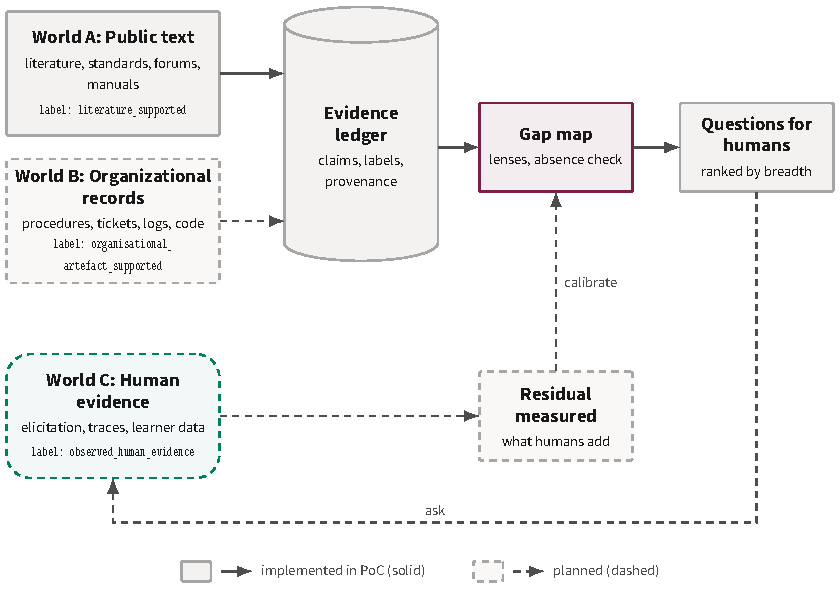
\includegraphics{figures/pdf/fig10_worlds.pdf}
  \caption[The three evidence worlds]{How public (A), organization-specific (B), and human (C)
    evidence interact. A and B build the reconstruction and the ledger; the gap map runs over the
    reconstruction and emits predictors; World C answers targeted questions and is the only path
    that can score those predictors, feeding back into the residual corpus that calibrates the
    next gap map. Solid arrows exist in the PoC; dashed arrows are future work.}
  \label{fig:worlds}
\end{figure}

\subsection{How evidence labels propagate}
\label{sec:platform-labels}

The six epistemic labels are defined in \cref{sec:evidence-model}. Four rules govern how a label
may move, all already enforced in the PoC or proposed as a direct extension of it:

\begin{itemize}[noitemsep]
  \item \textbf{Labels are computed, never set.} \code{ClaimRecord.label} is a property computed
    from a claim's evidence, not a field an author can assign (decision 0006) \evobs.
  \item \textbf{A label is only as strong as its weakest required link.} A claim is
    \code{literature_supported} only with a located span \emph{and} a cross-family
    \textsc{supports} verdict; a fabricated quote yields no evidence and the claim stays synthetic
    (decision 0007, rule \code{span-is-ours}) \evobs.
  \item \textbf{Derived outputs are \code{inferred} at best.} Gap records, gap-map scores,
    generated questions, recovered organizational rationale, and any domain-model edge a model
    proposes are \code{inferred} or \code{synthetic_extrapolation}, never higher \evobs{} for gap
    records (decision 0008 (proposed), rule \code{gap-candidates-are-predictors}), \evfut{}
    elsewhere. An evidential gate refuses a synthetic, inferred, or unknown
    criterion outright (\repo{residual/src/residual/gates.py}, decision 0006, rule
    \code{synthetic-never-a-gate-criterion}) \evobs.
  \item \textbf{Labels move up only through World C or cross-family verification, and World B
    labels stay inside their organization.} A human verdict can raise a claim to
    \code{observed_human_evidence}, and an \code{organisational_artefact_supported} claim must
    never leave its organization's tenant. Both rules have their types in the code today; neither
    is enforced yet \evfut.
\end{itemize}

\subsection{Components of the platform}
\label{sec:platform-components}

\Cref{tab:components} lists the platform's components. A status of \textsc{implemented in poc}
names the code that exists; \textsc{next research stage} names work planned inside the NOW
program (\cref{sec:roadmap}); \textsc{long-term} names work that depends on an organizational
partner, learner data, or a validated criterion that does not yet exist.

\begin{footnotesize}
\begin{longtable}{@{}p{0.17\linewidth}p{0.26\linewidth}p{0.24\linewidth}p{0.24\linewidth}@{}}
  \caption{Platform components: responsibility, status, and main technical risk. Component detail
    is in \repo{report/notes/06_platform.md}.}
  \label{tab:components}\\
  \toprule
  Component & Responsibility & Status & Main technical risk \\
  \midrule
  \endfirsthead
  \toprule
  Component & Responsibility & Status & Main technical risk \\
  \midrule
  \endhead
  \bottomrule
  \endfoot
  Reconstruction pipeline &
    Plan searches, fetch, extract claims bound to spans, hand off to verification &
    \evobs\ Walking skeleton, \repo{reconstruct/src/reconstruct/run.py} &
    Retrieval set by generator family; extraction truncation dropped sources once; validation
    deferred \\
  Evidence ledger &
    Single typed contract between stages: claims, evidence, sources, verifications,
    contradictions &
    \evobs\ \repo{residual/src/residual/ledger.py}; schema hash-frozen in
    \repo{residual/frozen/n1.json} &
    Run sidecar is a second, untyped contract; one JSON file per run does not scale to an
    organization's corpus \\
  Provenance verification &
    Every span a slice of fetched, hashed text; cross-family support verification; independence
    clustering &
    \evobs\ Open web only, \repo{reconstruct/src/reconstruct/evidence.py} &
    Decoy validity self-certified; short derived copies escape duplicate detection \\
  Contradiction analysis &
    Find claims that conflict across sources and worlds (A vs.\ B, imagined vs.\ done) &
    \textsc{Next research stage}: an older pairwise stage ran in the v1 runs; the current
    cross-verify stage is coded but has never run live (\repo{residual/src/residual/ledger.py},
    \cref{sec:n2}) &
    Scope-flagged contradictions can read as false conflicts; the detector must not be the
    generator \\
  Domain learning model &
    Hold the domain as a layered composite, not a single ontology &
    \textsc{Next research stage} / \textsc{long-term}. Only layer and knowledge-type enumerations
    exist &
    Prerequisite, causal, and procedural edges are not reliably recoverable from text alone \\
  Methodology-guided gap detection &
    Fire lenses where sources attest a construct but not its content; judge closure; emit gap
    candidates and retrieval gaps &
    \evobs\ Candidates only, \repo{gapmap/src/gapmap} &
    Closure judge uninformative: own rate equals mismatched-evidence-control rate on every ledger
    (\cref{sec:n3}) -- decides the program \\
  Company retrieval (World B) &
    Acquire organizational artifacts with dates, authorship, access rights, as fetchable,
    hashable text &
    \textsc{Next research stage} (public Git) / \textsc{long-term} (customer data). Nothing built &
    Access control ignoring per-user rights leaks data; injection via tickets/chat worse than via
    web pages \\
  Expert elicitation &
    Ask experts the gap map's questions by channel matched to knowledge type; one arm stays blind &
    \textsc{Long-term} for new tracks. Track A's instrument is frozen (\repo{instrument/}), reused
    only by copy &
    Anchoring on the reconstruction; an AI interviewer leading the expert; channel mismatch \\
  Human Knowledge Residual measurement &
    Recall of validated human answers against the reconstruction; unseen-item estimate with a
    known-truth check &
    \textsc{Next research stage}. Types exist; no estimator, no gold acquired &
    Never-written items are invisible to text checks; the matcher can become the gold it tests
    against \\
  EIG question selection &
    Choose the next question by expected information gain, reserving a fraction for
    confident-but-unverified areas &
    \textsc{Next research stage}. Current ranking is a breadth rubric, not information gain &
    No prior study applies EIG to expert/CTA interviews; adaptive selection breaks the
    equal-catchability assumption \\
  Learner diagnostics &
    Build bottleneck hypotheses from learner responses &
    \textsc{Long-term} (own data) / \textsc{next research stage} (public data). Vocabulary only &
    Synthetic learners are negative evidence for this role (\cref{sec:education}); AI Act
    Annex~III obligations \\
  Instructional design &
    Turn validated residual items into worked tasks and practice &
    \textsc{Long-term}. Nothing exists &
    Teaching an unvalidated candidate would teach a prediction as a fact (\cref{sec:education}) \\
  Adaptive learning &
    Sequence practice per learner from a learner model &
    \textsc{Long-term}. Out of scope for now &
    Unguarded model-generated help can raise assisted while lowering unassisted performance
    \parencite{bastani2025generative} \\
  Validation loops &
    End every stage in a pre-registered, code-computed continue/change/stop decision &
    \evobs\ Gates and checks exist; gold tests are \textsc{next research stage} &
    A threshold's registration source is free text, not enforced; several thresholds unset \\
  Run ledger and cost tracking &
    Log every model/search call, including failures, with cost and served-model checks &
    \evobs\ \repo{reconstruct/} per-run \code{calls.jsonl} &
    Cost per \emph{validated} item not yet tracked; needs World C \\
\end{longtable}
\end{footnotesize}

\begin{figure}[tbp]
  \centering
  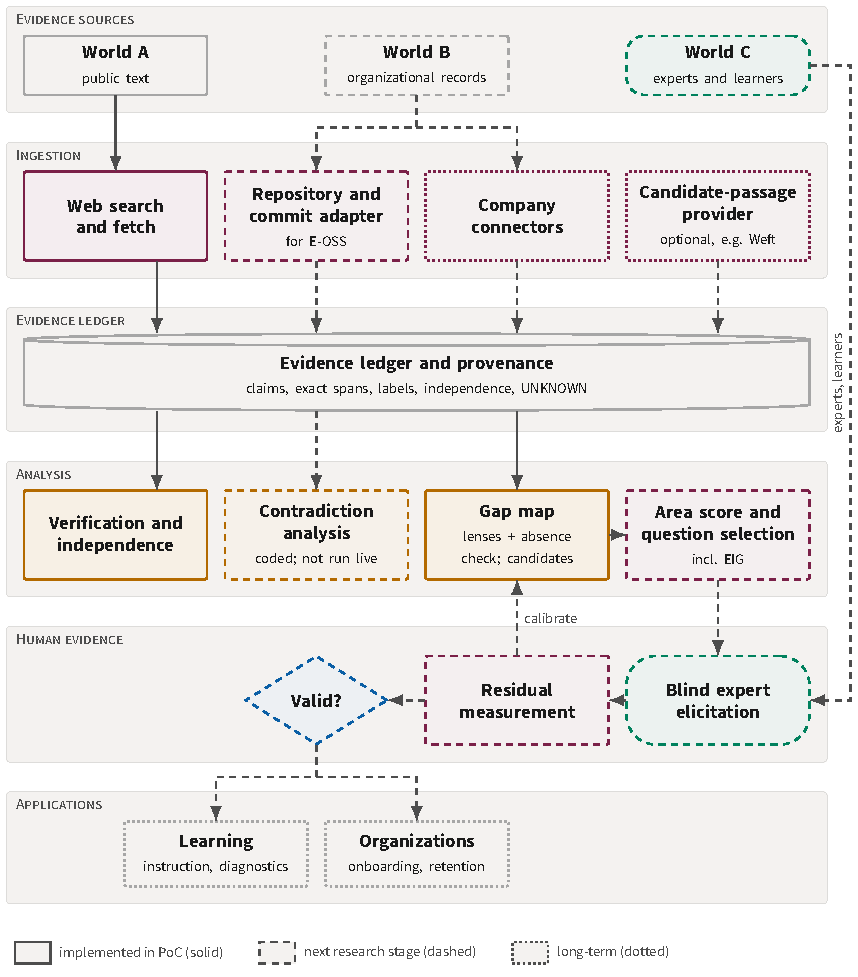
\includegraphics{figures/pdf/fig11_platform.pdf}
  \caption[Platform layers]{The platform drawn as layers, from evidence sources through
    acquisition, provenance, the evidence ledger, analysis, the human loop, and applications, with
    validation, audit, and security as a rail touching every layer. Solid boxes exist in the PoC;
    dashed boxes are the next research stage; dotted boxes are long-term. Every acquisition path
    passes through provenance before it reaches the ledger; only World C evidence can score the
    gap map's predictions.}
  \label{fig:platform}
\end{figure}

\subsection{Key architectural decisions}
\label{sec:platform-decisions}

Five decisions carry the platform's main design bets, drawn from
\repo{docs/architecture/decisions}. Two are already enforced in code: the evidence-ledger contract
and the synthetic-never-a-criterion gate. The three-model-family rule is followed today but checked
by code review, not by a test. The typed sidecar and the rule that unvalidated candidates never
reach a learner or end user are future work, the fifth adopted here for every application layer
that does not yet exist. Decision 0008, which the model-family and gap-candidate rules below draw
on, carries \code{status: proposed} in its own record.

\paragraph{The evidence ledger is the single contract between stages.}
Producers write typed records; consumers read them, and nothing else, so stages can be swapped or
re-run without touching each other. \evobs{} The core evidence package depends only on
\code{pydantic} (decision 0006, rule \code{residual-core-provider-neutral}). \evint{} One caveat:
the gap map also reads the reconstruction run's untyped JSON status sidecar, a second, informal
contract next to the ledger.

\paragraph{The run sidecar becomes a typed record.}
The platform closes that caveat by promoting run status into a schema with the same guarantees as
the ledger: versioned, hash-checkable, readable without re-deriving it from a log. \evfut.

\paragraph{Synthetic output may be a predictor, never a criterion.}
An evidential gate refuses a synthetic, inferred, or unknown label as the criterion side of any
measurement (decision 0006, rule \code{synthetic-never-a-gate-criterion}) \evobs. This is the
platform's main defense against a system that quietly grades its own predictions --- and why
\cref{sec:education} insists that only human-validated claims may reach a learner.

\paragraph{Three distinct model families for generator, verifier, and closure judge, on premises.}
The generator and verifier must come from different model families (decisions 0006, 0007) \evobs,
and the closure judge must differ from both again (decision 0008 (proposed)) \evobs. On-premises
deployment therefore needs three model families available locally, not one strong model reused
three times. The PoC already runs its closure judge locally (Ollama \code{qwen2.5:7b-instruct})
\evobs, showing the pattern is viable and, at the same time, its risk: that 7B judge did not beat
its mismatched-evidence control on any of the three PoC ledgers (\cref{sec:n3}).

\paragraph{Unvalidated candidates never reach a learner or an end user.}
A gap candidate is \code{inferred} by construction (decision 0008 (proposed), rule
\code{gap-candidates-are-predictors}) \evobs, and every application layer may only draw on claims
labeled \code{observed_human_evidence} or otherwise criterion-supported. \evfut{} No code enforces
this second part yet; it binds every future application layer.

\subsection{Non-functional requirements for organizational deployment}
\label{sec:platform-nfr}

Every requirement below is \evfut{}, stated as an extension of a property the PoC already has,
where one exists. Privacy, GDPR, and works-council requirements are stated once, in
\cref{sec:org-ethics}, and apply here unchanged; legal points there are the reorientation's own
reading of applicable law, not independently verified legal advice.

\paragraph{Security.}
Retrieved text is data, never instructions: the planner never sees artifact text directly,
extractors get no tool access, and injection-pattern spans are flagged and held pending rather
than acted on. This is already a rule for World A (decision 0007, rule
\code{retrieved-text-is-data}), extended to World B, where ticket and chat content is a stronger
injection vector than public web pages. Connectors use read-only, per-repository or per-space credentials, and any retrieval
substrate that runs third-party plugins in-process needs a pinned, reviewed allow-list, because an
in-process plugin runs with the adapter's own credentials to the organization's data
(\cref{app:weft}). One configured model backend per role, with a served-model check on every
response and no silent fallback list, holds for on-premises models exactly as it does today for
hosted ones (decision 0007).

\paragraph{Access control.}
Retrieval must enforce per-user access rights, and a claim inherits the most restrictive access
level of its supporting evidence. A gap map computed over restricted evidence is itself
restricted. World B claims never cross from one organization's ledger into another's, or into the
cross-organization residual corpus, without an explicit, contractual release and
de-identification. A reader without access to a claim's only supporting span must see that claim
as \code{unknown} for them, not as supported --- no type in the current schema expresses this yet.

\paragraph{On-premises models and audit trails.}
Organizational artifacts often cannot leave the premises they were created on. As
\cref{sec:platform-decisions} states, this requires at least three model families available
locally, one each for generation, verification, and closure judgment, following the pattern
already running for the N3 closure judge. Every model verdict is cached with its prompt hash and
replayed by default (decision 0008 (proposed), rule \code{gapmap-replays-by-default}), which
doubles as an audit and air-gapped-review mechanism. The PoC already logs every model and search
call, including failures, with the served model and its cost, snapshots that are
content-addressed, an offline re-slice of every evidence item, and a frozen schema and set of
prompt hashes (\repo{reconstruct/src/reconstruct/run.py}) \evobs. The platform adds: who viewed or
exported which gap map, which human verdict changed which label and when, and retention and
erasure events, all appended to a tamper-evident, hash-chained log. Cost headroom, including the
lesson the PoC's own budget stop taught, is stated once, in \cref{sec:resources}.

\subsection{Weft: a candidate substrate, not a dependency}
\label{sec:platform-weft}

Weft is a separate, public, MIT-licensed retrieval engine examined for this report as a possible
future World B acquisition layer; edu\_proj does not use, depend on, or integrate with it today.
It indexes a directory of text and PDF files with a content hash and a computed lineage. But it
keeps no in-document character offsets and no per-user access control, so any future adapter would
have to re-hash and re-locate every candidate passage itself, and never trust Weft's own chunk text
as a span. \Cref{app:weft} gives the full assessment: what Weft is today, why integration is not
justified now, the narrow candidate-passage role it could play at most as a long-term World B
component, and what must not be claimed about it.
